\epigraph{\emph{
  ``Everything should be built top-down, except the first time.''
}}{ Alan J. Perlis }
 
This section explains a general dataflow and the necessary steps to get data from an external source into a vectorized form. It will be held short giving intuition about a general setup, necessary preprocessing steps and as a point of reference what the Columbia Newsblaster system did. For the source code used throughout this thesis see the \href{https://github.com/sacry-/text-mining-haw-bachelor/}{News-Clusty Github repository}.

\section{Pipeline}
  
  A data pipeline for text data has various modules of interest. Where do we get the textutal content from? How is it stored? How is it preprocessed? What intermediate representations are useful? How do we handle the ongoing stream of input?

  \begin{figure}[h!]
    \centering
      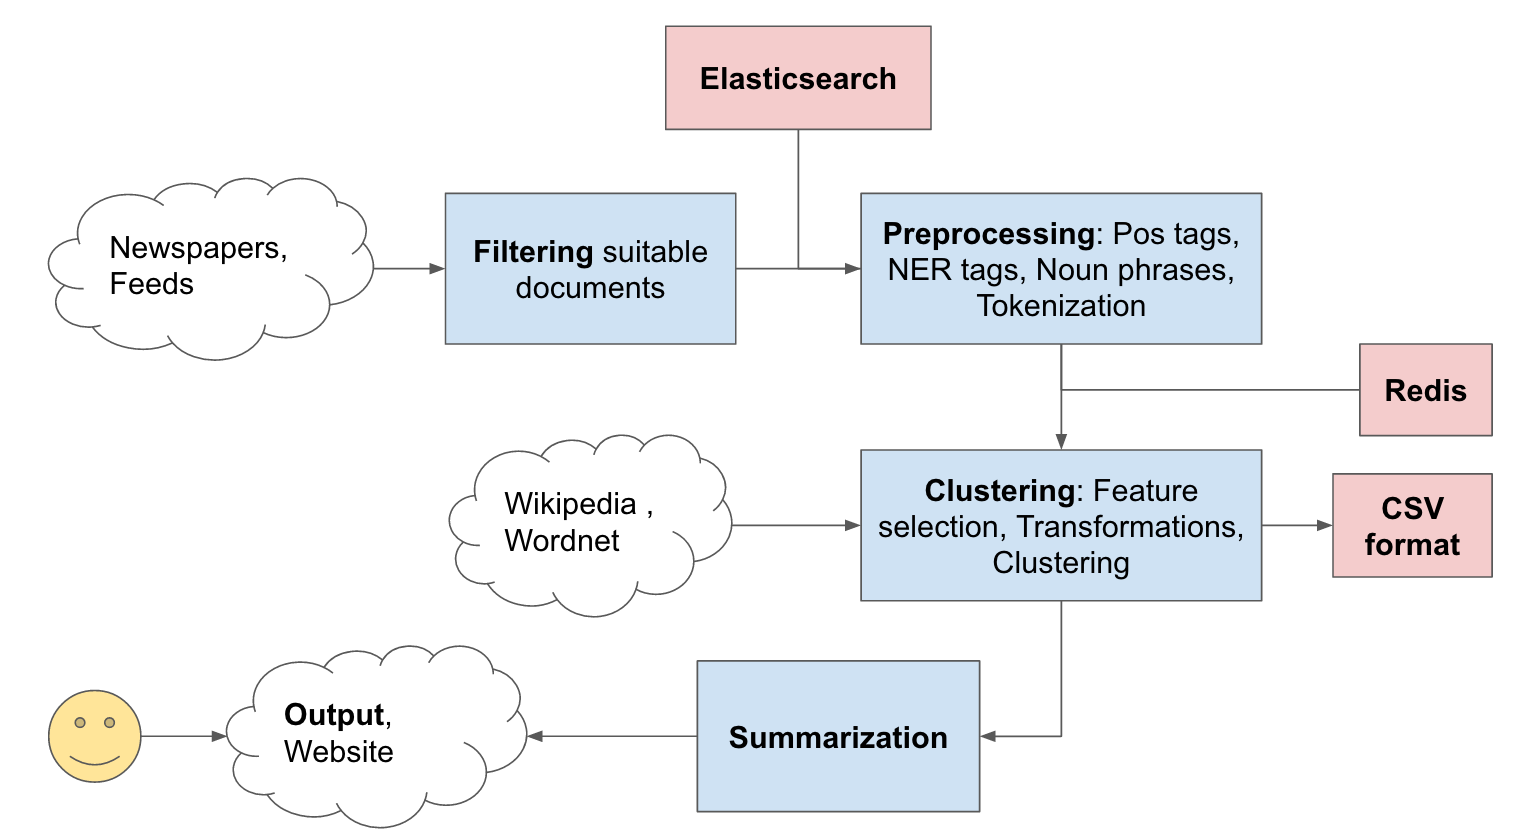
\includegraphics[width=0.7\textwidth]{news_clusty.png}
      \caption{"News-Clusty pipeline"}
      \label{news_clusty}
  \end{figure}

  The system that was developed for this thesis which is an early version is currently called ``News-Clusty''. Scraping, preprocessing and clustering are in place. There is a command line interface to interact with scraping and preprocessing. Currently it is an open question how to incorporate clustering schemes by a command line. The summarization and output generation is yet an open topic. The Columbia Newsblaster System by \cite{ColumbiaMultiDoc2001} is a very good point of reference. The core components of the Columbia Newsblaster are scraping, preprocessing, routing, clustering, summarizing and output generation. News-Clusty uses most of these components. They are briefly described in the following.

  \paragraph{Scraping} is the process of retrieving documents of interest in its raw form from websites, archieves and other sources. In the news domain we talk about online newspapers such as ``The Guardian'' or news feeds like google news. The inherent goal is then to persist the found pages. It is crucial to identify correct pages by several heuristics:

  \begin{enumerate}
    \item \emph{encoding} to utf-8 if working in english.
    \item \emph{language} to english, as a lot of newspapers have several languages to offer.
    \item \emph{content-length} has to be >= 500 chars to be relevant
    \item \emph{irrelevant content} like advertisement, not found pages, subscriptions etc.
  \end{enumerate}

  The more information one can collect about the article the better. Meta information like authors, meta keywords, keywords, categories, publishing dates, tags and links can be used later for more semantic strategies. Often meta keywords can completely contain what articles are about. These keywords can be reasonably used by looking up definitions on Wikipedia or Google, enhancing the content of an article. Publishing dates can be used to capture freshness by penalizing articles that are several days old.

  \paragraph{Preprocessing} is the step where raw content is send into a pipeline of filters until all noise and unnecessary information is stripped. In News-Clusty everything is on the internet in form of html pages. So a major task is to extract raw content from html to representative forms.\\
  In figure \ref{preprocessing} we work on two elastic search indices. The preprocessing module reads articles from the ``articles'' index, a continuous stream of documents and posts on the ``prep'' index. In the preprocessing we take all the actions listed and save the intermediate result as its own field. This is helpful later when computing expensive operations such as named-entity tags, noun-phrases or pos-tags. After processing the html we take a second filter step to make sure that the conditions of the scraping steps still hold true. If not the article is removed. Stripping html is not the only necessary step, we need to clean documents from bad characters, unuseful information we cannot work with like images. If the need arises spelling correction can be applied as well that is if there is sufficient evidence that articles have a lot gross misspellings, due to the central limit theorem this can be mitigated.

    \begin{figure}[h!]
      \centering
        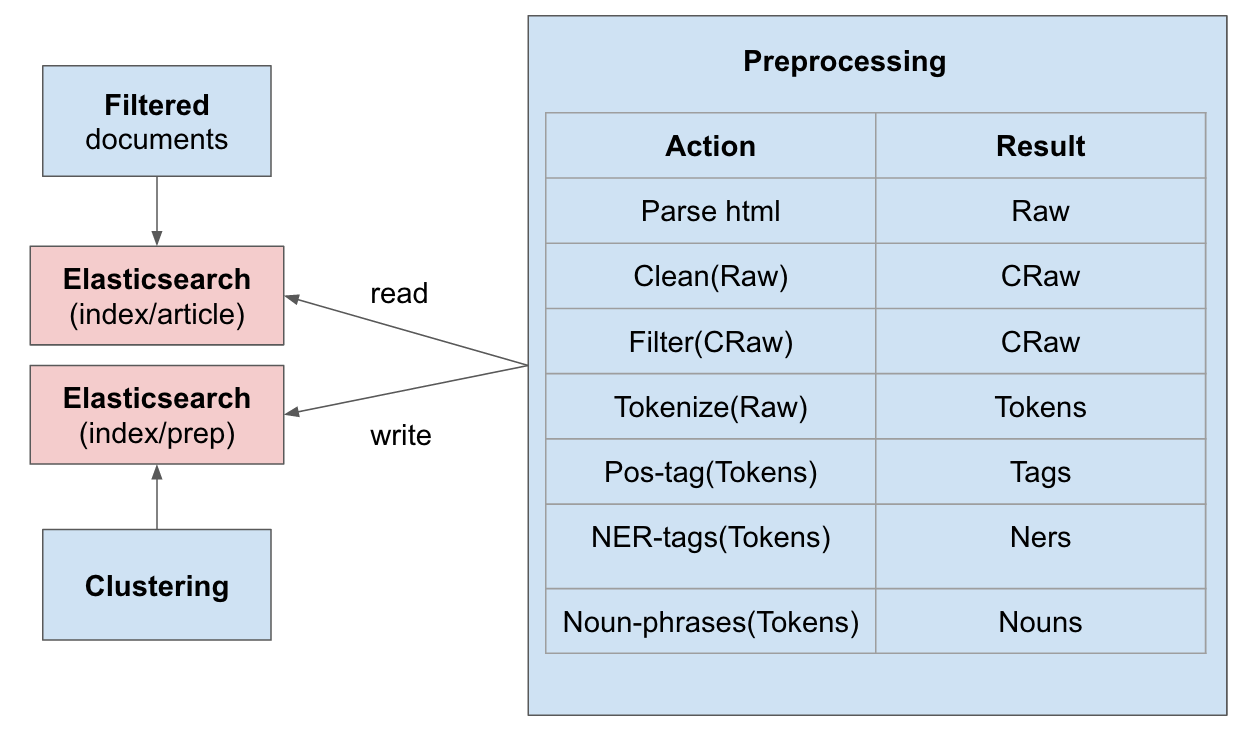
\includegraphics[width=0.7\textwidth]{preprocessing.png}
        \caption{"Preprocessing"}
        \label{preprocessing}
    \end{figure} 

  In figure \ref{preprocessing} ``Raw'' is the parsed text from the html, while ``CRaw'' represents text that contain no numbers, stopwords, short words, punctuations and special characters. The tokenization is not a whitespace splitter, it is a fully trained statistical parser that detects sentences and boundaries, as well as sentence tokens. The same goes for noun phrase extractors, pos-taggers and ner-taggers. ``CRaw'' is used as a representation of the text, while ``Raw'' is used to generate the beforementioned concepts.

  \paragraph{The Clustering} module does several transformations as displayed in figure \ref{clustering_cycle}. Feature selection is the process of picking features that are of most interest. This often happens mathematically by \emph{TF-IDF} or by formulas describing information density of words. If desired, resulting features can be enhanced by definitions and categories of \emph{Wikipedia} or projected via \emph{Wordnet} ontologies. Before the actual clustering algorithm is run similarity matrices and normalization to unit vectors is done. After this documents can be clustered by any kind of clustering algorithm. Outcomes are evaluated and redone if desired evaluation criterias were not met.

  \newpage
    \begin{figure}[h!]
      \centering
        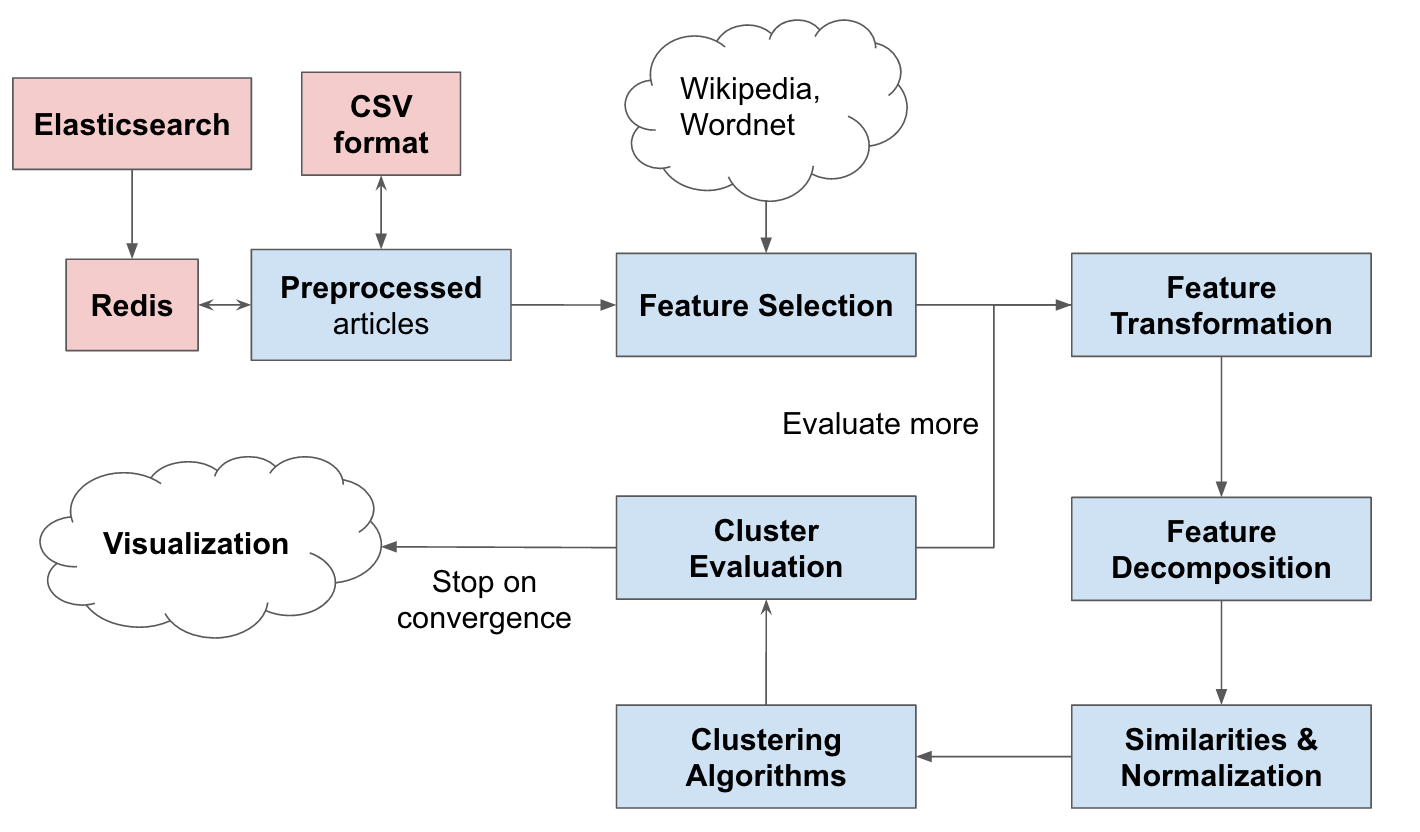
\includegraphics[width=0.7\textwidth]{clustering_cycle.png}
        \caption{"Clustering cycle"}
        \label{clustering_cycle}
    \end{figure} 

  \paragraph{The Summarization} module would receive the clustered documents as input. In addition meta information can be used here as well. The summarizer either gets single documents or a collection of documents that where in the same cluster. If assignments are soft, possible cluster overlaps can be taken into account. As this is not further part of the thesis we will leave it at that.

  \paragraph{Output generation} is a matter of visualizing the results of a summarization engine. For instance a website with rendered html. Currently clustering results can be projected to lower dimensions and to render 2D or 3D visualizations. Additionally the measures of clusterings can be compared and examined.

  \paragraph{The Routing engine} detects if the input is a type of event. They are categorized into ``single-events'', ``multi-events'', ``person-centered'' and ``other''. A single event is about the same topic e.g. the earthquake in Nepal 2015. Multi-events take place at different times, locations and with different subjects but with the same content, like terrorist attacks in 5 countries. A person-centered view is often a biography like a profile of Barack Obama running for president. This view makes it possible to make different assumptions about how articles should be summarized in case of the category of events that occured. A router like this could bring in various performance gains and strengthen the quality of a summarization. Due to time constraints this was left out of \emph{News-Clusty}.

\section{Python and Libraries}
  \emph{News-Clusty} is entirely written in the programming language Python and a well versed collection of libraries.

  \paragraph{Python} is a dynamic, object oriented higher level programming language with a rich environment for scientific computing. Python incorporates many different styles and assumptions, leading to a variety of programming paradigms between object oriented and functional programming. From the Zen of Python: ``Beautiful is better than ugly. Explicit is better than implicit. Simple is better than complex.''. For a proper introduction to Python see \cite{NltkPython}.

  \paragraph{The Persistence} of articles is held in \emph{Elasticsearch}. \emph{Elasticsearch} is a document store that can be easily distributed accross hundreds of nodes. It is schemaless and can be dynamically adjusted if need be. Its primary use case is for search and anything related to huge chunks of text. \emph{Redis} on the other hand is used as a cache for different feature selection strategies. It is a key value store and commonly chosen for fast execution. The common strategy is to first generate feature sets by querying \emph{Elasticsearch}. Each successful feature selection on a document will be persisted as a numerical feature vector into \emph{Redis}. Multiple accesses to the same documents will be read from \emph{Redis} if possible.\\
  While databases have huge advantages by querying documents, there is an overhead when accessing all files at once. If for a particular reason a whole dataset must be used, it is advised to use some of the serialization tools that output sparse matrix market formats or serializes to raw text files. Input and output on filesystems is faster if you do not need to query the data. This holds true as long as a single node filesystem is involved. \emph{Elasticsearch} for instance has its powers by leveraging clusters of servers (nodes).\\ 
  The indices for \emph{Elasticsearch} are scoped by the scraping date, $20150701/article/id = document$ or $20150701/prep/id = document$. This is particulary helpful if continuous processing, day by day, is an objective. The reason for choosing both is that we get highly expressive power and fast solutions for document queries and caching. If for several reasons the system should be setup in a distributed system of server nodes, both databases come with well defined abstractions.

  \paragraph{The Libraries} used throughout \emph{News-Clusty} are well-versed scientific data processing libraries. The library creators and maintainers should be mentioned and accredited for. \emph{News-Clusty} leverages linear algebra, feature selection strategies and clustering algorithms from \emph{Scipy} (especially numpy and sklearn) see \cite{ScikitLearn}. It uses natural language analysis tools from the nltk by \cite{NltkPython}. Moreover named entitiy recognition by the \emph{StanfordNLP group}, noun phrase extraction by \emph{Conll}, word ontologies by \emph{Wordnet}, knowledge and dictionaries by \emph{Wikipedia}. Additionally \emph{newspaper3k} for scraping newspaper articles and \emph{gensim} build by \cite{gensim2010} as high level abstractions for probabilistic topic models. In the future it would be good to rely less on certain libraries where it makes sense, e.g. not using \emph{newspaper3k} for scraping or \emph{Scipy} for clustering algorithms.



